\cotefile{31}
\scanpage{70}
\uline{Corollaire} Supposons que pour \unsure{tt.} \deleted{\unsure{partie}} \inserted{sous-schéma} fermé
\deleted{\unsure{irréductible}} $Y$ de $X$, et tt \deleted{$y\in Y$} \unsure{pt} \uline{\unsure{géom}}
$\bar y$ de $Y$, \unsure{les|l'} \unsure{anneau|anneaux} total des fractions $K_{Y,\bar y}$ de
$\underline O_{Y,\bar y}$ \deleted{\unsure{soit de|soient de} $\operatorname{cd}_{\ell}$} \unsure{satisfasse|satisfont} $\operatorname{cd}_{\ell}K_{Y,\bar y}\leq\dim\underline O_{Y,\bar y}$
$[=\dim\underline O_{Y,y}]$. \deleted{\uline{Alors} \unsure{soit} $\varphi$ \unsure{définie} \unsure{en}} [N.B. C'est \unsure{probablement}
tjrs. le cas, du moins si $X$ est ``bon''].

Posant pour \unsure{tt} \deleted{\unsure{e} $x\in X$ \unsure{partie} $Y$} $x\in X$
\[
\boxed{\varphi(x)=\sup_{y\in\bar x}\bigl(\operatorname{cd}_{\ell}(k(y))+2\dim\underline O_{\bar x,y}\bigr)}
\]
\deleted{Alors} et pour tte partie \inserted{fermée} $Y$ de $X$
\[
\deleted{\operatorname{cd}_{\ell}(X)\leq\unsure{?}}
\]
\[
\varphi(Y)=\sup_{y\in Y}\varphi(y)=\sup_{y\in Y}\bigl(\operatorname{cd}_{\ell}(k(y))+2\dim\underline O_{Y,y}\bigr)
\]
Alors
\[
\operatorname{cd}_{\ell}(X)\leq\varphi(X)
\]
% slanted
\margin{$\unsure{\psi|\varphi}(x)=\operatorname{cd}_{\ell}(x)+\deleted{\unsure{\sup_{y\in\bar x}}}\dim\unsure{\bar x|\bar X}_{\deleted{\unsure{y}}}$}

% slanted
\margin{\uline{Question} $A$ local noeth. hens. intègre, \unsure{de corps} résiduel $k$ \deleted{de dim \unsure{finie}}, tel que $\operatorname{cd}_{\ell}(k)<+\infty$. Alors $\operatorname{cd}_{\ell}K\geq\dim A+\operatorname{cd}_{\ell}k$\unsure{?} ??}

\uline{Exemples} 1) Schémas algébriques, plus \unsure{généralement|générlmt}
extensions résiduelles de degré de transcendance
\unsure{finies|finis|fini} [NB. ce degré de transcendance varie
simplement avec la dimension \ldots]

2) Corps de nombres

3) (conjecturalement) Ouvert de $\operatorname{Spec} A$,
$A$ \unsure{strictement} local

4) Schéma \unsure{alg.|rég.} \uline{affine} de dim 1
% archive sheet number: 69
\scanpage{71}
% Reversed type shows through from the other face.
\[
\deleted{\unsure{R}}\ i_*{\unsure{G|\mathcal G}}^{\unsure{d}}(\unsure{k|F})
\]
\[
H^*(G)\Longleftarrow E_2^{pq}=H^p(X,R^qi_*(G))
\]

\figure{\begin{tikzpicture}[x=.72cm,y=.74cm]
\draw (-1.25,0)--(9,0); \draw (0,-.4)--(.09,5.1);
\draw (.07,4.7)--(4.05,0);
\foreach \x in {0,.8,1.75,2.55,4.05,4.9,5.9,7,7.8}{\draw (\x-.08,-.11)--(\x+.08,.11) (\x-.09,.1)--(\x+.08,-.09);}
\draw (3.16,-.13)--(3.32,.13);
\foreach \y in {2.66,3.58,4.7}{\draw (.04,\y) circle (.075); \draw (-.04,\y-.10)--(.15,\y+.12);}
\foreach \x/\y in {2.94/1.30,3.44/.73}{\draw (\x-.06,\y-.10)--(\x+.07,\y+.10) (\x-.07,\y+.1)--(\x+.07,\y-.1);}
\node[below] at (4.03,-.08){$n-1$}; \node[below] at (4.91,-.09){$n$}; \node[below] at (5.92,-.1){$n+1$};
\end{tikzpicture}}
\[
x\in\operatorname{Supp}R^qi_*(G)
\]
\[
\deleted{\operatorname{cd}(\bar x)+\varphi(x)}
\]
\[
\deleted{\unsure{\varphi}}\quad \operatorname{cd}(\bar x)+q\leq
\]

\figure{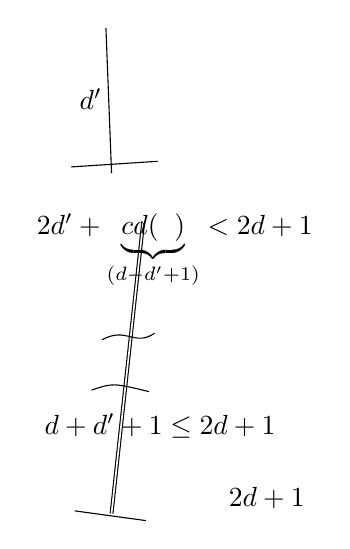
\begin{tikzpicture}[x=.65cm,y=.65cm]
\draw (0,-.18)--(-.11,2.65); \draw (-.79,-.06)--(.9,.05);
\node[left] at (0,1.26){$d'$};
\draw[double] (0,-6.83)--(.62,-1.12); \draw (-.72,-6.78)--(.67,-6.97);
\draw (-.39,-4.42)..controls (.03,-4.28)..(.73,-4.45);
\draw (-.19,-3.44)..controls (.29,-3.17) and (.44,-3.58)..(.84,-3.31);
\node[anchor=west] at (-1.65,-1.70){$2d'+\underbrace{\operatorname{cd}(\phantom{x})}_{(d-d'+1)}<2d+1$};
\node[anchor=west] at (-1.5,-5.12){$d+d'+1\leq 2d+1$};
\node[right] at (2.1,-6.52){$2d+1$};
\end{tikzpicture}}
\margin{$\deleted{\unsure{2d}}\ \leq d+1$ \unsure{?}\quad $1+2d'+(d-d'\deleted{\unsure{+1|2(d-1)}})=d+d'+1\leq 2d<2d+1$}

\[
\underline O_{X,\bar y}\otimes_X k(x)
\]
\[
\deleted{H^{\unsure{n|*}}(G)\mathbin{\unsure{-|\to}}H^{\unsure{n|*}}(\,}
\]
\[
\bullet\longrightarrow H^{n+1}(X)\longrightarrow H^{n+1}(G)
\]
\[
\deleted{q\leq\operatorname{cd}\underline O_{X,\bar y}\otimes}
\]
\[
q\leq\operatorname{cd}_p\operatorname{Frac}\underline O_{X,\bar y}
\]
\[
\underbrace{\operatorname{cd}(\bar y)}+q\,\underbrace{\operatorname{cd}_p\operatorname{Frac}\underline O_{X,\bar y}}<n\qquad y\in\bar x
\]
\[
\deleted{\varphi(y)<\varphi(x)-\operatorname{cd}_{\ell}(\,}
\]

\uline{Lemme}.
\[
\boxed{\begin{aligned}
&\operatorname{cd}_{\ell}(k(x))\leq n\\
&\forall Y\ \text{\unsure{vrai|rem|réunion} de } X,\quad \operatorname{cd}_{\ell}(Y)<n\\
&\forall y\in X,\ y\ne x,\quad \operatorname{cd}_{\ell}(\bar y)+\operatorname{cd}_{\ell}\operatorname{Frac}\underline O_{X,\bar y}<n
\end{aligned}}\ \overset{\displaystyle\operatorname{cd}_{\ell}(X)\leq n}{\nearrow}
\]
\[
2\dim\bar y+\underbrace{\dim\underline O_{X,\bar y}}_{\unsure{\in|\leq|\oplus}\dim\text{“}X-\dim\bar y}\qquad
\begin{aligned}\dim X+\dim\bar y&<\\&2\dim X\end{aligned}
\]
% archive sheet number: 70
\scanpage{72}
\mspage{\handwritten{6}}
morphismes fidèlement plats et quasi-compacts (cf Exp IV ,\handwritten{3.4.}), de plus
$Y=X/G$ est affine sur $S$. Si de plus $X$ est de présentation finie (resp.
de type fini) sur $S$, il en est de même de $Y$.

La première assertion résulte de Exp \handwritten{VIII} 5.1., \deleted{et de} traitant le cas où
$G$ est diagonalisable, et de Exp IV, \handwritten{3.5.2.}, qui permet de s'y ramener, compte
tenu que les morphismes fidèlement plats et quasi-compacts \inserted{$S'\handwritten{\to}S$} sont des morphismes de descente \uline{effective} pour la catégorie fibrée des schémas affines sur
d'autres, i.e. pour tout $Y'$ affine sur $S'$, muni d'une donnée de descente
relativement à $S'\handwritten{\to}S$, cette donnée de descente est effective, i.e. $Y'$
provient d'un $Y$ affine sur $S$, cf SGA VIII\deleted{\unsure{,}} 2.1. Pour la deuxième assertion, on est ramené également au cas diagonalisable\inserted{ Exp \handwritten{\unsure{VIII|VII}} 5.8.}, car les conditions de
finitude en\deleted{\unsure{g}}visagées se descendent par morphismes fidèlement plats et
quasi-compacts \deleted{(pour le type fini, c'est dans} (SGA VIII 3.3. et 3.6.). \deleted{Or,
dans ce cas, reprenant les notations de Exp VI 5.1., on aura $X=\operatorname{Spec}(\underline A)$,
$Y=\operatorname{Spec}(\underline A_{\unsure{o|0}})$, où $\underline A_o$ est l'algèbre formée \deleted{des} \inserted{la} composantes de degré 0
de l'Algèbre graduée $\underline A$.}

Procédant comme dans Exp V\handwritten{III}, corollaire\handwritten{s} 5.5.
à 5.7. , on tire de 2.3. :

\uline{Corollaire} 2.4. Sous les conditions de 2.3. , le morphisme graphe
\[
X\times_S G\handwritten{\longrightarrow}X\times_S X
\]
est une\handwritten{\unsure{/}}immersion fermée. Pour toute section $s$ de $X$ sur $S$, le morphisme
correspondant $g\handwritten{\leadsto}s.g$ :
\[
G\handwritten{\longrightarrow}X
\]
est une immersion fermée.

En particulier:

\uline{Corollaire} 2.5. Soit $u\mathpunct{:}G\handwritten{\to}H$ un monomorphisme de $S$-préschémas en groupes, avec $G$ de type multiplicatif et $H$ affine sur $S$. Alors $u$ est une
immersion fermée, \deleted{\unsure{et}} $H/G=Y$ existe et est affine sur $S$, \deleted{\unsure{E|e}}\unsure{e|E}nfin $H$ est un
fibré principal homogène sur $Y$ de groupe $G_Y$.
% archive sheet number: 71
\scanpage{74}
\uline{Théorème 1}$_n$ Soit $A$ anneau str. local noeth., de dim $n$, \inserted{\deleted{\unsure{str. excellent}} satisfaisant cond. de \unsure{finitude|stricte}}
\deleted{alors pour tout} \inserted{$Y=\operatorname{Spec}(A)$} $F$ un faisceau de $\ell$ torsion sur
$X=\operatorname{Spec} A[t]$, \inserted{$\ell$ premier à la car. résiduelle,} tel que $x\in\operatorname{Supp} F\Longrightarrow\dim\underline O_{X,x}\geq m$.
(en un mot ; $F$ est ``nul en codim $<m$). \deleted{Dans
ce cas \unsure{si|où} \unsure{moins|montre} \illegible{1} \unsure{que} en plus \unsure{que} support \unsure{en codim} \unsure{pour} \unsure{le pt gén.} de $X$}.
Alors $H^i(X,F)=0$ pour $i>n+1-m$.
% slanted
\margin{\uline{Question} Est-il \unsure{nécessaire} que $F$ soit de torsion ???}
[En particulier, $\operatorname{cd}_{\ell}(X)\leq n+1$\deleted{\unsure{]}} , et pour tte partie fermée $Z$
de $X$, \deleted{de codim} $\operatorname{cd}_{\ell}(Z)\leq n+1-\operatorname{codim}(Z,X)$]

\uline{Théorème} $2_n$ Soit $A$ anneau str. local noeth de
dim $n$, \deleted{et $f\in A$} $X=\operatorname{Spec}(A)$, $f\in A$, $U=X_f$, Alors
$\operatorname{cd}_{\ell}(U)\leq n$ pour tout $\ell$ premier à la car. résiduelle.

[N.B. $1_n\Rightarrow2_n$ car on plonge $U$ comme fermé \inserted{de codim $\geq1$,} dans $Y[t]$.]

\uline{Lemme 1} $\underbrace{2_{n'}\ \text{pour }n'\leq n+1}_{2'_{n+1}}\Longrightarrow 1_n$
\inserted{(aussi $=1_{n'}$ \unsure{pour} $n'\leq n$ i.e. $1'_n$)}. En effet, on est ramené à
prouver que si $S\subset X$ fermé est de codim $m$,
alors $\operatorname{cd}_{\ell}(S)\leq n+1-m$. \inserted{On \unsure{peut supposer} $S$ irréd.} Or soit $\bar S$ l'adhérence de
$S$ dans $\bar X=\mathrm P^1_Y$, considérons $T=\bar S-S$, c'est un
schéma str. local ($\subset\bar X-X$), soit $x$ son pt fermé.
Cons. \deleted{pour} \inserted{\unsure{tout|pour}} $F$ de $\ell$-torsion sur $S$
\[
H^i(\bar S,F)\longrightarrow H^i(S,F)\longrightarrow H_T^{i+1}(\bar S,F)
\]
Or
\[
\begin{aligned}
H^i(\bar S,F)&=H^i(\bar S_0,F)=H^i(\mathrm P^1_k,F_0),\ (\text{nul si }i\geq3)\\
H_T^{i+1}(\bar S,F)&=H^i(\bar S_x-T_x,F_{(x)})\qquad\text{si } i\geq2
\end{aligned}
\]
\deleted{nul par l'hyp. \unsure{de}}
D'ailleurs $\dim\bar S_x\leq n+1-m$ car \deleted{\unsure{rien|bien}}
% archive sheet number: 73
\scanpage{75}
\unsure{S|Si} Car \deleted{en localisant aux pts génériques}
\[
\dim\bar S_x+\underbrace{\operatorname{codim}(\bar S_x,\bar X_x)}_{\geq m}\leq\dim\bar X_x=n+1
\]
donc par l'hyp. \deleted{de récurrence} $2_{n'}$ pour $n'\leq n+1$
[en particulier $2_{n+1-m}$], on conclut
\[
H_T^{i+1}(\bar S,F)=0\quad\text{si }i>n+1-m.
\]

\uline{Si} $n+1-m\geq2$, \inserted{i.e. $m\leq n-1$,} on a de \unsure{$=$}
\[
H^i(\bar S,F)=H^i(\bar S_0,F_0)\ =\ 0\quad\text{si }i>n+1-m\geq2
\]
d'où $H^i(S,F)=0$. Reste le cas
$m\geq n$, \inserted{donc ($S$ étant $\ne\varnothing$) $m=n$ ou $n+1$} \deleted{Si $m\geq n+1$,} \inserted{\deleted{Si $m=n$, et} Si $m=n+1$,} alors $S$ est \deleted{un pt}
vide ou une \deleted{\unsure{et partie de}} \inserted{partie finie de} $X_0$, et on a
bien $H^i(S,F)=0$ pour $i>0=(n+1)-m$, OK.

Si $m=n$, alors \deleted{le \unsure{seul cas}} \unsure{ch. que|chaque} comp.
\deleted{irréductible \unsure{de}} $S$ est de dim $\leq1$. \deleted{Pour les
\unsure{comp.} irréductibles qui ne sont pas
$=X_0$,} \inserted{Si $S\ne X_0$} on a $\bar S_0$ de dim 0, donc
$H^i(\bar S_0,F)=0$ si $i>0$, à fortiori si $i>n+1-m=1$.

Pour $S=X_0$, on est ramené à prouver
que sur un corps sép. clos \unsure{$k$, ]} son $k\unsure{(t)|[t]|(x)}$ est de \deleted{dim. \unsure{coh|cd}} $\operatorname{cd}_{\ell}\leq1$,
ce qui est connu.
% archive sheet number: 74
\scanpage{76}
\uline{Lemme} 2 Se bornant aux anneaux
ess. de type fini sur un corps, on a
\[
\deleted{1^{\unsure{'+|\prime}}_n\Rightarrow 2'_{n+2}}.\qquad 1'_n+2'_{n+1}\Rightarrow2'_{n+2}
\]
[N.B. Et $2'_{n+2}\Rightarrow1'_{n+1}+2'_{n+2}$ grâce au lemme 1, OK]

En effet, on est sur un corps (sép clos $k$).
\deleted{et \unsure{le dernier|la dernière} de $f\in\unsure{\sqrt{0}} A$} \inserted{On peut supposer dans $2'_{n+2}$ que}
$f\in\unsure{\sqrt{0}|\not\sqrt{0}|\mathfrak m}A$ (sinon $X_f=\varnothing$ et tt est trivial]
\figure{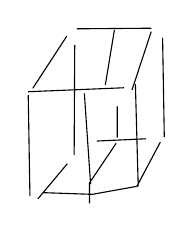
\begin{tikzpicture}[scale=.72]
\draw (0,.07)--(-.03,1.85) (.05,1.97)--(.65,2.89) (.83,3.02)--(2.14,3.03);
\draw (-.03,1.91)--(1.66,1.98) (1.33,2.03)--(1.49,3.00) (1.8,1.94)--(2.14,2.97);
\draw (2.34,2.86)--(2.37,1.11) (2.30,1.02)--(1.88,.23) (1.86,2.05)--(1.91,.24);
\draw (.14,.02)--(.66,.64) (.22,.13)--(1.10,.10)--(1.88,.24) (1.05,-.06)--(1.05,.30)--(1.52,1.00) (1.07,.28)--(.96,1.88);
\draw (.78,.79)--(.79,2.73) (1.18,1.04)--(2.05,1.08) (1.54,1.1)--(1.54,1.65);
\end{tikzpicture}}

\deleted{Alors $f$ \unsure{définit}} On peut supposer $A$
intègre si on y tient. Complétons
$f$ en un système de paramètres
\figure{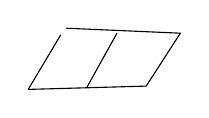
\begin{tikzpicture}[scale=.7]
\draw (.02,0)--(.61,.99) (.71,1.11)--(2.78,1.02)--(2.16,.06)--(.02,0);
\draw (1.08,.03)--(1.63,1.02);
\end{tikzpicture}}
$f_1=f,\unsure{f_1|f_2},\ldots f_{n+2}$, \deleted{les $n+1$ premiers}
\inserted{qui} définissent \deleted{$A_1=k\langle x_1,\ldots,x_n,\rangle\to A$}
$A'=k\langle x_1,\ldots x_{n+2}\rangle\to A$, Et $X$ \deleted{$=\operatorname{Spec}$}
est fini sur $X'=\operatorname{Spec} A'$, $U$ est l'image
inverse de $U'=X'_f$. On est
ramené à prouver que $\operatorname{cd}_{\ell}(U')\leq n$. Donc on
peut supposer $A=k\langle x_1,\ldots x_{n+2}\rangle$, \inserted{$f=x_1$.} Considérons
$B=k\langle x_1,\ldots x_{n+1}\rangle$ qui est de dim $n+1$, et
soit $Y=\operatorname{Spec} B$, $U=Y_f$. Considérons la projection
$V\longrightarrow U$. Par l'hyp. \deleted{de} $2'_{n+1}$, il suffira de
prouver que \deleted{\unsure{$f$}} $R^qf_*(F)$ est nul en
codim $i\unsure{\leq|<}q-1$, car alors $H^p(U,R^qf_*(F))\ne0$
$\Rightarrow\deleted{\unsure{pour}}\ p\leq n+1-(q-1)$. i.e. $p+q\leq n+2$,
d'où $H^i(V,F)\ne0\Rightarrow i\leq n+2$.

% slanted
\margin{Attention : \unsure{condition|conditions} \unsure{un|en} \unsure{moins} ?}
% archive sheet number: 75
\scanpage{77}
Or les anneaux locaux des pts de $U$ sont
de dim \uline{$i\leq n$} ! Donc de $=$ les anneaux
strictement locaux $B'$ de $U$, et \deleted{\unsure{de}} $V$ étant
affine de dim. relative 1 sur $U$, donc
$V'=\unsure{V|B}\otimes_B B'$ \inserted{affine et} de dim relative 1 sur $B'$, on
\unsure{conçoit|constate|consort} que l'hyp $1'_n$ va impliquer
que $H^{\deleted{\unsure{p}}q}(V',F')=0$ si $q>i+1$ i.e. \uline{$i<q-1$},
[i.e. $R^qf_*(F)$ est nul en codim $i<q-1$].
C'est ce qu'il faut vérifier, \unsure{pièce|prière|rien} \unsure{en|au}

\uline{Lemme 3} $1'_n$ \deleted{\unsure{étant}} \inserted{[\deleted{\unsure{est}} pour des ess. t.f. sur corps]}
implique que
pour tt préschéma affine $X$, \unsure{ess.t} de
t. f. sur un corps sép. clos $k$, $X$ de
dim de Krull $d\leq n+1$, on a $\operatorname{cd}_{\ell}(X)\leq\dim X$

\uline{Dém} Par passage à la limite, on peut supposer
que $X$ est de t. f. sur $k$. \inserted{Récurrence sur $d=\dim X$, $d\leqn+1$} \deleted{Par lemme}
\inserted{Trivial si $d\leq0$. \deleted{Par lemme} soit donc $d\geq1$.} Par lemme
de normalisation, on peut supposer $X={\unsure{\mathbb E|\mathrm E}}^d_k$.
\inserted{($d\leq n+1$) : prouver $\operatorname{cd}_{d}(\mathbb E^d_k)\leq d$}
\deleted{Récurrence sur $d\leq n+1$.} Trivial si $d\leq0$.

En \unsure{projetant|général}, $X=\mathbb E^d_k\mathrel{\overset{f}{\unsure{-|\longrightarrow}}}Y=\mathbb E^{d'\deleted{\unsure{-1}}}$, où $d'=d-1\leq n$.
En vertu de $1'_n$, $R^qf_*(F)_{\bar y}\ne0$
$\Rightarrow\deleted{\unsure{dim}}\ q\leq\dim\underline O_{Y,\bar y}+1\deleted{\unsure{=q+2|i+1}}\inserted{=i+1}$. i.e. $R^q f_*(F)_{\bar y}$ est
% archive sheet number: 76
\scanpage{78}
``nul en codim $<q-1$''. Par l'hyp. de récurrence
il s'ensuit que $H^p(Y,R^qf_*(F))\ne0\Rightarrow$
\margin{$n-q+1$}
$p\leq n-(q-1)$ \unsure{ou} i.e. $p+q\leq n+1$. Donc $E_2^{pq}=0$
sauf si $p+q\leq n+1$, d'où la conclusion\ldots

Par suite, les th. 1 et 2 sont prouvés
dans la situation \deleted{``\unsure{ess.|loc.} t.f. sur}
``\deleted{ponct. \unsure{ess.|est}}\inserted{\unsure{E-ponctuellt|E-ponctuellement}} t.f. sur $k$''. Il en est
donc de \unsure{$=$} pour le lemme 3, de \unsure{$=$}
pour ``ess. de t.f. sur $k$''.
% slanted
\margin{\uline{\unsure{Concl.}}}

Nous allons maintenant le prouver
\unsure{également|a fortiori} quand il s'agit de préschémas
\unsure{E-ponctuellement} de t.f. sur un
anneau \inserted{\uline{noeth}} $\Lambda$ \uline{de dim $\leq1$}. Nous le
prouvons sous \uline{\unsure{sa|ses} forme locale} $2_n$,
par \uline{récurrence sur} $n$, trivial si $n=0$,
on peut supposer $n>0$, et le th. démontré
pour $n'<n$. On peut supposer $\Lambda$ \uline{str. local}
\inserted{intègre} \uline{de dim 1}, $\Lambda\to A$ \deleted{et} \inserted{local} \deleted{intègre \uline{dominant} $\Lambda$,} \inserted{injectif.}
% slanted
\margin{\uline{Arranger la} \uline{démonstration}}
% slanted
\margin{\uline{Récurrence} \uline{inutile}}
% archive sheet number: 77
\scanpage{79}
\diagram{\begin{tikzcd}[ampersand replacement=\&]X\arrow[d]\\Y\end{tikzcd}}
\figure{\begin{tikzpicture}[scale=.78]
\draw (0,1.58)..controls (-1.78,1.49) and (-1.65,-1.55)..(.05,-1.55)..controls (2.12,-1.51) and (1.95,1.55)..(0,1.58);
\draw (-1.44,-.10)..controls (-.4,-.21) and (.58,-.15)..(1.51,-.23);
\draw (.06,1.59)..controls (-.13,.92) and (.08,.25)..(.14,-.15)--(.16,-1.42);
\draw (.08,1.43)..controls (.81,1.32) and (.50,.14)..(.14,-.15);
\fill (.14,-.15) circle (.09);
\node[above] at (.16,1.64){$V(\pi)$};\node[right] at (1.52,-.24){$V(f)$};
\node[left] at (-1.48,1.08){$V\,\bigl\{$};
\draw (-1.44,-4.94)--(1.39,-5.02); \fill (-.13,-4.97) circle (.08);
\end{tikzpicture}}

Soit $\pi\in\unsure{\mathfrak r|r|\mathfrak m}\Lambda$, $\pi\ne0$ donc $\pi$
non div. de 0, \deleted{Alors \illegible{1}} \inserted{Posons}
\[
\deleted{H^{i}_{\unsure{*}}\quad\unsure{V'|V}=X_f}
\]
\[
V=X_f,\quad U=X_{f\pi}=V_{\pi},
\]
\deleted{Alors}
\[
Z=V-U=V\cap V(\pi)=V(\pi)_f,\quad \text{Alors}
\]
\diagram{\begin{tikzcd}[ampersand replacement=\&,column sep=large]
H_Z^i(V,F)\arrow[r]\& H^i(V,F)\arrow[r]\& H^i(U,F)\arrow[ll,bend right=24]
\end{tikzcd}}
et il suffit de prouver que les extrêmes
sont nuls pour $i\geq n+1$. Or $U$ est affine de dim
$\leq n-1$, \inserted{ponct. de t.f.} sur le corps des fractions $K$ de $\Lambda$,
\margin{\#} donc (\unsure{réf|ilf}) $K$ est de dim coh $\leq1$, et
par suite $U$ est de $\ell$-dim ch. $\leq(n-1)+1=n$,
\deleted{D'autre part} ce qui dispose du dernier terme.
Pour le premier, on a
\[
H_Z^*(V,F)\Longleftarrow H^p(Z,\overbrace{\underline H_Z^q(F)})
\]
Or \deleted{je dis que} comme $Z=V(\pi)_f$, \inserted{est sur $k(\Lambda)$,} on
dispose de la dim ch. de $Z$ (qui est
$\leq n-1$) et de ses sous-schémas fermés.

Les termes $E_2^{pq}$ pour $q\ne0,1$ ne donnent
pas de contribution aux $H_{\unsure{?|Z}}^i(V,F)$ pour $i\geq n+1$.
\deleted{Reste} Or je dis que de façon générale
% archive sheet number: 78
\scanpage{80}
\[
\underline H_Z^q(F)_{\bar x}\ne0\ \longrightarrow\ \dim\underline O_{Z,x}\deleted{\unsure{\leq}}\geq q-1
\]
i.e. $\underline H_Z^q(F)_{\bar x}$ est nul en codim $<q-1$,
[ce qui impliquera que $H^p(Z,\underline H_Z^q(F))\ne0\longrightarrow$
$p\leq(n-1)-(q-1)=n-q\deleted{\unsure{+1}}$ i.e. $p+q\leqn\deleted{\unsure{+1}}$, d'où
la conclusion voulue]. Il faut donc prouver que $q-1>\dim\underline O_{Z,x}\deleted{\unsure{+1}}\mathrel{\unsure{=|\Rightarrow}}\underline H_Z^q(F)_{\bar x}=0$.
Pour $q=0,1$, c'est \unsure{vide|évid|évidemment}. Sinon, on a
\[
\underline H_Z^q(F)_{\bar x}=H^{q-1}(X_{\bar x}-V(\pi)_{\bar x}\deleted{\unsure{d}},F),
\]
qui est \inserted{bien} nul
si $q-1>\dim X_{\bar x}$ [car \inserted{$X_{\bar x}$} c'est un
affine ess. de t.f. sur un corps sép. clos $\unsure{\bar K|K}$]
\deleted{de dim}
% slanted
\margin{\uline{\unsure{Calcul|Couac|Comme}} \uline{d'une} \uline{unité}}

\deleted{\uline{Question}} \inserted{\uline{Th}} Soit $A$ \uuline{str.} local, \inserted{$Y=\operatorname{Spec} A$, $Y'=Y-\{\unsure{m|\text{pt}}\}$,} $X$ \inserted{\unsure{aussi|ass.}} de type fini
et affine, \deleted{de dim de Krull} \inserted{$X'=X\times_Y Y'$}
Soit \deleted{\unsure{$d\leq$|$X_0$}} $d=\sup[\dim X_0,\ \dim X'+1]$.
Alors est-il vrai que pour tt $\ell$
premier à la car. rés. de $A$, on a
\[
\deleted{\unsure{H^i}}\ \operatorname{cd}_{\ell}(X)\leq d
\]
% slanted
\margin{Prouvé pour l'instant pour les anneaux ess. de type fini sur un anneau de dim $\leq1$}

\inserted{N.B. Si $X$ est intègre et domine $Y=\operatorname{Spec} A$ [ce qu'on peut tjrs supposer) on trouve $\operatorname{cd}_{\ell}(X)\leq\dim Y+d$ \inserted{$d=\dim$ de la fibre générique}}

N.B. Si on ne suppose pas $X$ affine, la formule serait
\[
\operatorname{cd}_{\ell}(X)\leq\sup[2\dim X_0,2\dim X'+1]
\]
\margin{\deleted{$\unsure{A\to Y}$,}}
resp. ($X$ irréd dominant) $\operatorname{cd}_{\ell}(X)\leq2\dim Y-1+2d$ \inserted{(si $\dim Y\ne0$)}
% archive sheet number: 79
\scanpage{81}
\diagram{\begin{tikzcd}[ampersand replacement=\&]\unsure{\mathbb E|\mathrm E}=Y[t_1,\ldots t_{\unsure{r}}]\arrow[d,no head]\\Y\end{tikzcd}}
On peut supposer $Y$ intègre, \inserted{de dim $\unsure{n|\varphi}$,} $X$
plongé dans $\mathbb E\mathrel{\unsure{:|=}}Y[t_1,\ldots,t_r]$, $X$ intègre.
\deleted{Alors codim} Je dis que
\[
\operatorname{Codim}(X^{\unsure{\prime}},E)\geq n+r-\unsure{\delta|d|\nu}\quad\text{i.e. }\delta\geq\inserted{n+r-}\operatorname{codim}(X,E)
\]
En effet, si $X\ne X_0$, alors le premier membre est
égal à $\operatorname{codim}(X',E')\unsure{=}\dim E'-\dim X'$
% slanted
\margin{\unsure{tt|H} sur un ``bon'' Jacobson $Y'$}
\[
=((n\unsure{-}1)+r)\deleted{\unsure{+}}-\dim X'\geq(n-1+r)-(\delta-1)=n+r-\delta\quad\text{OK}
\]
Si $X=X_0$, alors $\delta$\deleted{$\unsure{\geq\sup(}=\dim X_0-$}
\[
\begin{aligned}
\operatorname{Codim}(X,E)&=\operatorname{Codim}(X_0,E_0)+\operatorname{Codim}(E_0,E)=\\
&=(r-\delta)+n\qquad\text{OK.}
\end{aligned}
\]
[NB. On \inserted{ne} peut avoir $\operatorname{codim}(X,E)>n+r-\delta$,
\deleted{sauf} \inserted{que} lorsque $\dim X_0>\dim X'+1$ \deleted{\unsure{pour}} \inserted{mais}
\deleted{\unsure{ou}} $X\ne X_0$.]
\margin{\uline{est-ce possible ?} \uuline{non}}
\deleted{Or, puisque $X_0\ne\varnothing$, \unsure{de} utilisant la formule des dimensions,}
\inserted{\unsure{Non.|N.B.} prouvons en fait}
\margin{\deleted{\unsure{$H^i$}} $\operatorname{cd}_{\ell}(X)\leq(n+r)-\operatorname{codim}(X,E)$}

On va procéder par récurrence sur $r$.
Pour $r=0$, c'est trivial \deleted{(tt est [\unsure{str}} (alors $X\subset Y$, donc $H^i(X,F)=0$ pour $i>0$ i.e.
$\operatorname{cd}(X)=0\leq\deleted{\unsure{r-n}}n\unsure{-|\geq}\operatorname{codim}(X,Y)=\dim X$. Si
$r=1$, c'est le th. $1_n$. Dans le cas
\deleted{général}, \inserted{$r\geq2$} on utilise la suite spectrale
pour $E_Y^r\longrightarrow E_Y^{r-1}$ \ldots\ldots
% archive sheet number: 80
\scanpage{82}
\uline{Question} $X$ schéma noeth \uuline{affine},
\[
n=\sup_{x\in X}\bigl[\operatorname{cd}_{\ell}(k(x))+\dim\underline O_{X,x}\bigr]
\]
\inserted{$\ell$ premier aux car. rés.}. Alors
$n$ est aussi le Sup des $\ell$-dim coh. des
ouverts affines de $X$. La partie \unsure{vache|ardue} est
\[
\operatorname{cd}_{\ell}(X)\leq n
\]

Mais c'est faux déjà pour l'anneau
des entiers d'un corps de \unsure{nbres}
\unsure{car|où} on a \uline{$n=2$} s'il est \deleted{\unsure{pur}} tot. imag.,
alors que $\operatorname{cd}(X)=3$ !
% archive sheet number: 81
\scanpage{83}
Dim coh. d'un schéma affine sur $\mathbb Z$

\diagram{\begin{tikzcd}[ampersand replacement=\&]X\arrow[d,"f"]\\\operatorname{Spec}(\mathbb Z)=\unsure{S|\mathbb S}\end{tikzcd}}
$\deleted{\unsure{p}}\ell 1_X$ \uline{inversible} i.e. $\ell\notin f(X)$, \uline{$\ell\ne2$}.
Supposons \unsure{d'abd|d'ab.} $X$ intègre \inserted{\unsure{dominant|domine} $S$} dim relative $d$
\[
H^*(X,F)\Longleftarrow H^p(S_{\ell},R^q f_*(F))
\]
\[
R^q f_*(F)_{\unsure{\eta|g|\mathfrak g}}\ne0\ \Longrightarrow\ q\leq\deleted{\unsure{d+1|1+}}d
\qquad(\unsure{\eta|\mathfrak g}\ \text{\unsure{le pt} gén})
\]
\[
R^q f_*(F)_s\ne0\ \Longrightarrow\ q\leq1+d
\]

Donc si $q>1+d$, on a $E_2^{pq}=0$. 

si $q=1+d$ alors $R^q f_*(F)_{s}$ est concentré \unsure{aux|sur des|sur les} pts fermés
donc $E_2^{pq}\ne0\Longrightarrow p\leq1$

Si $q\leq d\deleted{\unsure{+1|+d}}$ alors $E_{2}^{pq}\ne0\longrightarrow p\leq2$

\figure{\begin{tikzpicture}[x=.64cm,y=.63cm]
\draw (-.73,-.02)..controls (2,.00) and (4.8,.28)..(6.75,.15);
\draw (.08,-.9)--(-.05,5.0);
\node[above] at (-.10,5.37){$q$}; \node[right] at (7.42,-.12){$p$};
\node[left] at (-.07,3.75){$1+d$}; \node[left] at (-.05,3.00){$d$};
\foreach \x/\y in {0/0,.95/.04,1.97/.07,0/.66,.99/.76,1.97/.85,0/2.34,1.02/2.37,1.95/2.40,0/3.06,.94/3.09,1.98/3.12,0/3.72,.91/3.78}{\draw[thick] (\x-.07,\y-.09)--(\x+.07,\y+.09) (\x-.08,\y+.06)--(\x+.07,\y-.05);}
\end{tikzpicture}}

On trouve donc
\[
\begin{aligned}
\operatorname{cd}_{\ell}(X)&\leq d+2=\dim X+1\\
&\phantom{\leq d+2}=\operatorname{cd}'_{\ell}R(X)
\end{aligned}
\]
\deleted{\unsure{Cette}} \unsure{ce|la} formule est valable
si $X$ est concentré \deleted{au} dessus
d'un point $p$ de $S=\operatorname{Spec}(\mathbb Z)$. Donc on
trouve en tous cas si \uline{$X$ affine} de t.f. sur $\mathbb Z$,
$\ell 1_X$ inversible, et $\ell\ne2$ \uline{ou} $X_{\mathbb Q}$ \deleted{\unsure{domi|devrait}} est au
dessus d'un corps \inserted{tot.} imaginaire,
\[
\boxed{\operatorname{cd}_{\ell}(X)\leq\dim X+1}\deleted{=\unsure{\operatorname{cd}}}
\]
% archive sheet number: 82
\scanpage{84}
% Broad pencil strokes cancel this entire face. The smaller cancellations are local.
\deleted{\uline{Théorème} 3.1. Soient $S$ un \deleted{pré}schéma affine, $\deleted{G}\handwritten{H}$ un $S$-groupe de type multiplicatif, $F$ un faisceau quasi-cohérent sur $S$, sur lequel $G$ opère (Exp 1,
4.7.) Alors \deleted{pour tout $i\quad0$, la cohomologie de Hochschild} on a}
\[
\deleted{H^i(\deleted{G}\handwritten{H},F)=0\qquad\text{pour }i\quad0,}
\]
\deleted{où $H^{\unsure{\bullet|\prime|i}}$ est la cohomologie de Hochschild étudiée dans Exp.1 5.}

\deleted{En effet, d'après loc cit , 5.3. , la cohomologie de Hochschild
s'explicite, en\deleted{\unsure{t}} termes des\deleted{\unsure{it}} anneaux affines $A$ de $S$ et $B$ de $G$, et du
\deleted{\unsure{mo}} module $M$ sur $A$ définissant $F$, comme cohomologie d'un complexe
\deleted{$C^{\unsure{n|p|*}}(G,F)$, dont la} de $A$-modules $C^{\unsure{\circ|\bullet}}(\deleted{G}\handwritten{H},F)$ , \uline{dont la formation commute au
changement de base} $A\quad A'$ . Par suite, pour un changement de base
$A\quad A'$ avec $A'$ \uline{plat} sur $A$, on aura}
\[
\deleted{H^i(\deleted{G}\handwritten{H}',F')=H^i(\deleted{G}\handwritten{\unsure{H|G}},F)\otimes_A A',}
\]
\deleted{et par suite, si on suppose même $A'$ fidèlement plat sur $A$, pour prouver
que $H^i(\deleted{G}\handwritten{H},F)$ est nul, il suffit de prouver qu'il en est ainsi de $H^i(G',F')$.
Cette remarque nous ramène à vérifier 3.1. dans le cas où $G$ est diagonalisable, dans ce cas cela a été prouvé dans Exp 1 5.3.3.}

\deleted{Utilisant les résultats de Exp.III , nous allons tirer de 3.1.
diverses conséquences de nature géométrique:}

\deleted{\uline{Théorème} 3.2. Soient $S$ un \deleted{pré}schéma\deleted{, $G$ un groupe de typ} affine, $S_{\unsure{o|0}}$
un sous-schéma affine défini par un Idéal $J$ \uline{de carré nul} , $\deleted{G}\handwritten{H}$ un groupe
de type multiplicatif sur $S$, $\deleted{H}\handwritten{G}$ un \deleted{\unsure{g}}préschéma en groupes quelconque sur $S$,
$u,v:\deleted{G}\handwritten{H}\quad\deleted{H}\handwritten{G}$ deux homomorphismes de groupes tels que $u_o=v_o$ , où
$u_o,v_o\mathrel{\unsure{\mathbin{:}|=}}\deleted{G}\handwritten{H}_o\quad\deleted{H}\handwritten{G}_o$ sont les homomorphismes déduits de $u,v$ par changement de
base $S_o\quad S$. Alors il existe un $g$ \deleted{\unsure{$G$}} $\in$ \inserted{$G(S)$} tel que $v=\operatorname{int}(g)\ u$ \handwritten{et $g_o=e$.}}

\deleted{Cela résulte de Exp III \qquad et de 3.1.}
% archive sheet number: 83
\scanpage{85}
\uline{Conjectures sur la cohomologie des schémas affines}

\margin{\unsure{1}}
$X$ : (``bon'') schéma affine intègre pt gén. $\unsure{\alpha|x|a}$.
$\ell$ \unsure{nb} premier

$1^\circ$) Si $\ell 1_X$ inversible, alors
\[
\operatorname{cd}_{\ell}(X)\leq\operatorname{cd}_{\ell}(k(x))
\]
\margin{\deleted{\unsure{[}} [et cela devient une égalité pour les ouverts assez petits ?]}

$2^\circ$) Si $\ell 1_X$ non inversible et non nilpotent, on a
\[
\operatorname{cd}_{\ell}(X)\leq\sup\bigl(\operatorname{cd}_{\ell}(k(x)),\unsure{\delta|\nu}(V(\ell))+3\bigr)
\]
où on pose, pour un schéma $Z$ de car. $\ell$
\[
\delta(Z)=\sup_{\substack{z\ \text{maximal}\\\text{de }Z}}\delta(k(z))
\]
et pour un corps $k$ de car $\ell$
\[
\delta(k)\quad\text{tel que}\quad \ell^{\delta(k)}=[k:k^\ell]
\]

\deleted{$1^\circ$ bis) Sous \unsure{la condition|les conditions} de $2^\circ$, lorsque $\exists\ \ell'$ \deleted{\unsure{un}} \inserted{premier} tel
que $\ell'1_X$ inversible i.e. $X$ sur $S_{\ell'}$ ($S=\operatorname{Spec}\mathbb Z$),
alors on peut remplacer \inserted{dans la formule}
$(\delta(V(\ell))+3)$ par $\delta(V(\ell))+1$. Sous les conditions
de $2^\circ$, lorsque}
% slanted
\margin{\deleted{\uline{Question} A-t-on tjrs $\operatorname{cd}_{\ell}(k(x))\unsure{\geq|>}\delta(V(\ell))+1$}}

Supposons $\exists$ \deleted{\unsure{un entier}}\inserted{$\ell'$}
premier tel que $\mathbb Z_{\ell'}$ inversible. Alors
\[
\operatorname{cd}_{\ell}(X)\deleted{\unsure{\leq\sup(}}\inserted{\leq}\operatorname{cd}_{\ell}(k(x))\deleted{\unsure{,\delta(V(\ell))+1)}}
\]

$4^\circ$) $A$ bon anneau local hensélien intègre, \unsure{cor.|car.} \unsure{résiduel|résiduelle} $\unsure{k|\ell}$,
car $K=0$. Soit $U$ ouvert affine de $X=\operatorname{Spec} A$. Alors
\[
\operatorname{cd}_{\ell}(U)\leq\dim A+\delta(k)+\operatorname{cd}_{\ell}(k)
\]
% archive sheet number: 84
\scanpage{86}
% archive sheet number: 85
% Face upside down in the scan. Long oblique cancellation strokes cover the typescript.
\deleted{\deleted{\unsure{Notons}} Notons en passant le résultat suivant, qui servira dans un exposé ultérieur:}

\deleted{\uline{Corollaire} \handwritten{4.6.} Soient $X$ un $S$-préschéma plat, $U$ une partie ouverte de $X$, on suppose que pour tout $s\handwritten{\in} S$, $U_s$ est schématiquement dense dans $X_s$.
Supposons de plus que $X$ est localement noethérien, \uline{ou} $X$ localement de présentation finie sur $S$ et $U$ rétrocompact dans $X$ (ou ce qui revient au même, $U$ de présentation finie sur $X$; il suffit par exemple $X$ et $U$ de présentation finie sur $S$).
Alors $U$ est schématiquement dense dans $X$.}

\deleted{Le cas $X$ localement noethérien n'est mis que pour mémoire, il est contenu dans \handwritten{4.3.} Dans le deuxième cas envisagé, on peut évidemment
supposer $S$ et $X$ affine, alors $X$ et $U$ sont de \unsure{présentattion|présentation} finie sur $S=\operatorname{Spec}(A)$. \inserted{$A$ est limite inductive de ses sous-$\underline{Z}$-algèbres $A_i$ de type fini.} Le ``procédé bréveté'' déj\unsure{è|e|à} utilisé (explicité en long et en
large dans EGA IV 8) montre qu'il existe un \deleted{schéma noethérien affine} \deleted{\unsure{et un anneau|et un|sous-anneau}} 
$i$, un schéma affine $X_i$ sur $S_i=\operatorname{Spec}(A_i)$ et un ouvert
$U_i$ dans $X_i$, dont $X,U$ se déduisent par changement de base \deleted{\unsure{et|de|si}} $S\quad S_i$.
\deleted{Pour tout $j\quad i$,} soit $E_{\deleted{\unsure{j|i}}\handwritten{i}}$ la partie de $S_{\handwritten{i}}$ formée des $s\quad S_{\handwritten{i}}$ tels que $U_{\handwritten{i}\,s}$ soit schématiquement dense dans $X_{\handwritten{i}\,s}$. Cette condition signifie aussi
 que $U_{\handwritten{i}\,s}$ contient \deleted{\unsure{les|le}} l'ensemble $\operatorname{Ass}\,\underline{O}_{X_{\handwritten{i}\,s}}$ des points ``associés'' au faisceau structural de $X_{\handwritten{i}\,s}$, et les résultats de EGA IV 9 montrent
alors que cette condition est de nature constructible, i.e. que $E_{\handwritten{i}}$ est une partie constructible de $S_{\handwritten{i}}$. D'ailleurs, la question envisagée sur
les fibres est invariante par extension du corps de base, ce qui prouve \deleted{\unsure{que pour $k,j,$|que pour $k$|que pour tout $j$}\illegible{2}} \inserted{en vertu de l'hypothèse faite que} 
l'image inverse \inserted{$\handwritten{\unsure{E|=}}$} de $E_{\handwritten{\unsure{i|j}}}$ par $S_{\deleted{\unsure{k|j}}}\handwritten{\longrightarrow} S_{\handwritten{\unsure{i|j}}}$ \deleted{\unsure{par que|part que|part}} est
$S$, et entraine par EGA IV 8 qu'il existe un $j\handwritten{\geq}i$ tel que l'image
inverse \deleted{\unsure{de|le}} $E_j$ de $E_i$ dans $S_j$ soit $S_j$, i.e. que pour tout $s\handwritten{\in}S_j$, $U_{j\,s}$ est schématiquement dense dans $X_{j\,s}$. 
En vertu de 4.4. appliqué à $(\unsure{S|E}_j,X_j,U_j$ et au\deleted{\unsure{x}} changement de base $S\handwritten{\to} S_j$, il s'ensuit que $\unsure{U|X}$ est schématiquement dense dans $X$.
On notera d'ailleurs qu'on n'utilise ici 4.4. que dans le}
% Last line ends at the edge after « le ».
